\section{BanditMF: Multi-Armed Bandit Based Matrix Factorization Recommender System}
The authors in \cite{billsus2000user} proposed a method that is based on implicit and explicit user feedback, agents use machine learning algorithms to inscribe an individual user model and use the user model to make recommendations. The method called BanditMF, a matrix factorization recommendation system based on multi-arm bandit, is proposed to address the limitations of collaborative filtering and bandit algorithms as mentioned earlier. The system combines model-based collaborative filtering matrix factorization (MF) with a multi-armed bandit algorithm. BanditMF incorporates an offline subsystem centered on matrix factorization and an online subsystem focused on a multi-armed bandit algorithm.

\begin{minipage}{\textwidth}
        \begin{minipage}[t]{0.45\textwidth}
            \centering
            \makeatletter\def\@captype{table}\makeatother
            \begin{tabular}{llllll}
\hline
                       & $i_{1}$ & $i_{2}$   & $i_{5}$   & $i_{4}$   & $i_{5}$   \\ \hline
\multicolumn{1}{l}{$u_{1}$} & 1.4      & ?   & 1.1 & 0.7 & ?   \\
\multicolumn{1}{l}{$u_{2}$} & ?        & 0.3 & ?   & 0.7 & 0.5 \\
\multicolumn{1}{l}{$u_{3}$} & 0.4      & 0.3 & ?   & ?   & 0.3 \\
$u_{4}$                     & 1.4      & ?   & 1.2 & ?   & 0.8 \\ \hline
\end{tabular}
\caption{User-item rating matrix}
        \end{minipage}
        \begin{minipage}[t]{0.45\textwidth}
        \centering
        \makeatletter\def\@captype{table}\makeatother
\begin{tabular}{llllll}
\hline
                       & $i_{1}$ & $i_{2}$   & $i_{5}$   & $i_{4}$   & $i_{5}$   \\ \hline
\multicolumn{1}{l}{$u_{1}$} & 1.4      & 0.8   & 1.1 & 0.7 & 0.9   \\
\multicolumn{1}{l}{$u_{2}$} & 1.0       & 0.3 & 1.0   & 0.7 & 0.5 \\
\multicolumn{1}{l}{$u_{3}$} & 0.4      & 0.3 & 0.3   & 0.1   & 0.3 \\
$u_{4}$                     & 1.4      & 0.7   & 1.2 & 0.8   & 0.8 \\ \hline
\end{tabular}
\caption{Predicted rating matrix}
        \end{minipage}
    \end{minipage}

By analyzing the user-item rating matrix as shown in Table 3.1, we can obtain the predicted user-item rating matrix as shown in Table 3.2.
For the sake of explanation, we consider each row in Table 3.2 as a predictive model. In another world, we consider the row vectors that represent the preferences of each user as models. When a new user enters the system, a predictive model is selected and used as a basis to make recommendations for the new user. However, in the real world, the number of users is generally in the millions, so the above approach is rendered impractical due to the $m\times n$ scaling rating matrix, where the $m$ is millions of orders in size. 

\begin{figure}[htbp]
\centering

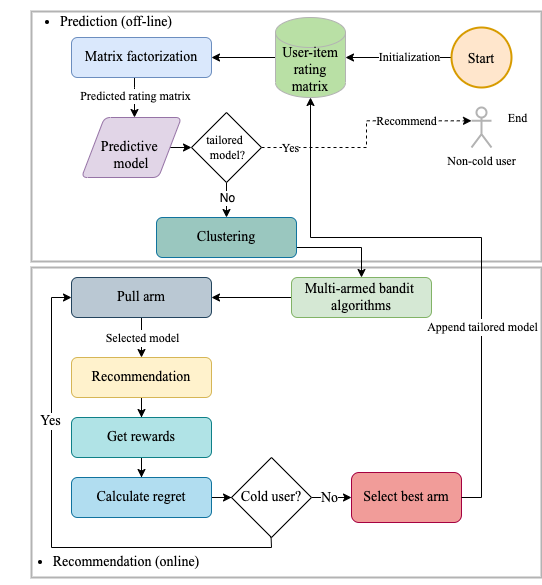
\includegraphics[scale=0.8]{figure/fc.png}
\caption{Flow chart of the BanditMF}
\end{figure}

Whether we can cluster the rows in the matrix to reduce the size of the rating matrix(i.e., reduce the number of predictive models)? Inspired by collaborative filtering, it is possible to cluster the rows of the rating matrix such that each row of the matrix represents a row vector, and each row vector represents the preferences of each user, so that each cluster is composed of users with similar rating preferences. Another important reason for matrix factorization is the very widespread assumption that the user-item rating matrix is a low-rank matrix, so the clustering can be performed on the rows of the user-item rating matrix. We treat BanditMF as an algorithm consisting of two stages: (1) prediction, and (2) recommendation.

For the offline subsystem, we define the prediction model as the following steps: matrix factorization based rating prediction, clustering, and unified rating

\textbf{\textit{Matrix factorization based rating prediction}}. As we illustrated in section 3.1, the non-cold user formed the user-item rating matrix $ R $and, based on the matrix factorization, we can get the predicted user-item rating matrix $\hat{R}$. The notation $\hat{r}_{u,i}$ is used to represent the rating of user \textit{u} on item \textit{i}. Recall that in this project, our predicted rating is:
\begin{equation}
    \hat{\boldsymbol{r}}_{u,i}=b_{u,i}+q_{i}^{T} * p_{u}
\end{equation}
And the loss function is:
\begin{equation}
    \operatorname{Loss}=\min _{q^{*}, p^{*}} \sum_{(u, i) \in K}\left(r_{u,i}-b_{u,i}-q_{i}^{T}p_{u}\right)^{2}+\lambda \left(\left\|q_{i}\right\|^{2}+\left\|p_{u}\right\|^{2}+b_{u}^{2}+b_{i}^{2}\right)
\end{equation}
where $b_{u,i} = \mu+b_{u}+b_{i}$. We use $\mu$ denote the average rating for the entire rating matrix, $b_{u}$ denote the user's bias, and $b_{i}$ is represent the item bias.

\textbf{\textit{Clustering}}. According to the user’s preference vectors of the predicted user-item rating matrix $\hat{R}$, we can perform the clustering on the row of the $\hat{R}$.  In this system, \textit{K-means} algorithm is adopted, which is measured by \textit{Euclidean distance}. After performing the clustering on the user’s preference vectors, we will have a set of clusters where $\mathcal{C}=\left \{ c_{1},c_{2}\cdots c_{n} \right \}$.

\textbf{\textit{Unified rating}}. For the clusters in $\mathcal{C}$, we perform the average rating on it to get the unified user preference vectors, where $\hat{\alpha}$ denote the unified user preference vectors. For example, as shown in Table 3.3, by the hypothetical that $u_{1}$ and $u_{2}$ be clustered into $ c_{1}$, the unified user preference vectors $ \hat{\alpha}=\left \{ 1.2,0.55, 1.05,0.7, 0.7 \right \}$, which is the average of the $u_{1},u_{2}$.

\begin{table}[htbp]
    \centering
\begin{tabular}{llllll}
\hline
  & $i_{1}$ & $i_{2}$   & $i_{5}$   & $i_{4}$   & $i_{5}$   \\ \hline
$u_{1}$& 1.4      & 0.8   & 1.1 & 0.7 & 0.9   \\
$u_{1}$& 1.0       & 0.3 & 1.0   & 0.7 & 0.5 \\ \hline
$\hat{\alpha}_{1}$& 1.2      & 0.55 & 1.05   & 0.7   & 0.7 \\

\end{tabular}
\caption{Unified user preference vectors}
\end{table}
The online recommendation module is mainly composed of multi-armed bandits, and this online module runs as follows:
\begin{itemize}
    \item[1. ] Select a predictive model $\mathcal{S}_{n}$ using the MAB algorithm $\pi$
    \item[2. ]  Select and recommend the item $i^*$ with the top rating score in $\hat{\alpha}$ which is not recommended to user $u$.
    \item[3. ]  Receive the user $u$'s rating for item $i^*$.
    \item[4. ]  calculate the reward and regret.
    \item[5. ]  Determine whether a user is a cold user by a threshold $\tau $.
    \item[6. ]  If yes, update the algorithm $\pi$. Otherwise, turn to the offline module.
\end{itemize}
The online recommendation module will provide recommendations to new users until the new user is no longer cold (i.e., some feedback on the recommended items or preferences has been provided to the system). Nevertheless, if a system obliges the user to make excessive ratings, the user will lose interest in the system \cite{threshold}. For the above reasons, we cannot run the bandit algorithm too many times to get the optimal recommendation, and online systems need to get user preferences in a limited number of recommendations(i.e., within the threshold $\tau $).

Now let's walk through the entire BanditFM workflow from scratch, which is the flowchart shown in Figure 3.5. The input information is first fed into the offline prediction module, and through matrix factorization, we get the predicted user-item rating matrix. Then each row of the matrix, namely the user preference vector, is clustered to reduce the size of the prediction matrix. If we denote the original size predicted user-item rating matrix as $m\times n$, after clustering, we have a ${m}'\times n$ matrix, where ${m}'\ll m$. Then pass the clustered predictive model to the online recommendation module. Through the multi-armed bandit algorithm, it selects the predictive model from the clusters. Get user preferences through interaction with users (i.e., an algorithm recommends items to users and users provide feedback). The online module determines whether a user is a cold user through a threshold $\tau $, and if the system has collected certain user rating preferences, then the user is no longer a cold user. At this point, we switch to the offline prediction module and append the user preferences obtained from the online module to the user-item rating matrix. We can then accurately make recommendations to new users through the matrix factorization technique.

\textbf{\textit{Reward and Regret}}. In BanditMF, we define the \textit{reward} as the equation shown in the formula 3.23.
\begin{equation}
    \mu_{\mathcal{S}_{n}}\left ( t \right ) =\frac{r_{u,i}}{r^*}
\end{equation}
where $r^*$ denote the maximum rating in the dataset. $r_{u,i}$ denote the rating of user $u$ for recommended item $i$ according to the algorithm selected predictive model $\mathcal{S}_{n}$. The reward interval is $\mu_{\mathcal{S}_{n}}\left ( t \right )\in [0,1]$.This intuition of this reward can be interpreted as the higher the feedback received for the recommendation, the higher the reward will be. If by the reward, then we define the \textit{regret} as:
\begin{equation}
    R(T) \triangleq \sum_{t=1}^{T}\left(\mathbb{E}\left[\mu^*\right]-\mathbb{E}\left[\mu_{\mathcal{S}_{n}}\left ( t \right )\right]\right)
\end{equation}
where $\mathbb{E}\left[\mu^*\right]$ denotes the maximum expected cumulative rewards.

In the next chapter, we will verify the BanditMF using various criteria and compare the performance of different multi-armed bandit algorithms.